\documentclass{article}
\usepackage{ctex}
\usepackage{bm}
\usepackage{enumitem}
\usepackage{mathrsfs}
\usepackage{subcaption}
\usepackage{graphicx}
\usepackage{amsmath,amsthm,amsfonts,amssymb}
\DeclareMathOperator{\sinc}{sinc}
\DeclareMathOperator{\rect}{rect}
\newtheorem{definition}{定义}
\newtheorem{thm}{定理}
\newtheorem{pro}{命题}
\newtheorem{cor}{推论}
\def\P{\textbf{P}}
\def\E{\mathbb{E}}
\def\Var{\textrm{Var}}
\def\Cov{\textrm{Cov}}
\begin{document}
\title{信号检测理论}
\author{赵丰}
\maketitle
\begin{enumerate}
\item Bayes 准则

定义似然比为$\lambda(z) \triangleq \frac{p(z|H_1)}{p(z|H_0)}$
\begin{equation}
\lambda(z)\mathop{\gtreqless}_{z\in \mathcal{Z}_0}^{z\in \mathcal{Z}_1} \lambda_B(z)\triangleq \frac{P(H_0)(C_{10}-C_{00})}{P(H_1)(C_{01}-C_{11})}
\end{equation}
其中$C_{ij}=P(D_i,H_j)$

\item 极大极小准则(先验概率$\xi=P(H_0)$未知),满足极大极小化方程:
\begin{equation}
C_{00}P(D_0|H_0)+C_{10}P(D_1|H_0)=C_{01}P(D_0|H_1)+C_{11}P(D_1|H_1)
\end{equation}
解出$\xi_{MM}$,根据
\begin{equation}
\lambda(z)\mathop{\gtreqless}^{z\in \mathcal{Z}_1}_{z \in \mathcal{Z}_0} \lambda_{MM} \triangleq \frac{\xi_{MM}(C_{10}-C_{00})}{(1-\xi_{MM})(C_{01}-C_{11})}
\end{equation}
设计接收机。
\item Neyman Pearson 准则:
给定 $P_F=\alpha$,使得$P_D$最大。
\begin{equation}
\lambda(z)\mathop{\gtreqless}^{z\in \mathcal{Z}_1}_{z \in \mathcal{Z}_0} 
\lambda_{NP}
\end{equation}
其中 $\lambda_{NP}$满足方程
\begin{equation}
P_F=\int_{z\in Z_1}p(z|H_0)dz=\alpha
\end{equation}

\item ROC曲线:将由Neyman Pearson 准则计算出的$(P_F,P_D)$曲线。

\item 在理想白高斯信道中信号的检测

考虑高斯带限白噪声,即
\begin{equation}
S_N(f)=\begin{cases}
0 & \textrm{if } |f|>B\\
\frac{N_0}{2} & \textrm{if } |f|<B
\end{cases}
\end{equation}
可以证明$S_N(f)$对应的相关函数是$R_N(\tau)=\frac{N_0\sin(2B\pi \tau)}{2\pi \tau}$

\begin{proof}
首先已知$\mathcal{F}(\sinc(t))=\rect(f)$
其中
$$
{\displaystyle \mathrm {rect} (f)={\begin{cases}0&{\mbox{if }}|f|>{\frac {1}{2}}\\{\frac {1}{2}}&{\mbox{if }}|f|={\frac {1}{2}}\\1&{\mbox{if }}|f|<{\frac {1}{2}}.\\\end{cases}}\quad\sinc(x)=\frac{\sin(\pi x)}{\pi x}}
$$
根据Fourier变换的性质:若$\mathcal{F} f(x)=\hat{f}(\lambda)$,则$\mathcal{F}f(ax)=\frac{1}{a}\hat{f}(\frac{\lambda}{a})$
因此$\mathcal{F}(\sinc(2Bt))=\frac{1}{2B}\rect(\frac{f}{2B})$,等式两边同时乘以$N_0B$得
$\mathcal{F}(N_0B\sinc(2Bt))=\frac{N_0}{2}\rect(\frac{f}{2B})$
\end{proof}
由相关函数的性质
$R_N(0)=N_0B$为高斯分布的方差。

可以证明,若$n(t)$是高斯带限白噪声随机过程,在$[0,T]$时间内,关于$z_i(t)=s_i(t)+n(t),i=0,1$的信号检测似然函数为:
\begin{equation}
\lambda(z(t))=\exp\left(\frac{2}{N_0}\int_0^T (s_1(t)-s_0(t))z(t)dt -\frac{1}{N_0}(\int_0^T (s_1^2(t)-s_0^2(t))dt)\right)
\end{equation}

接收机工作性能

设随机变量$v=\int_0^T [s_1(t)-s_0(t)]z(t)dt$,根据最小平均错误概率准则
\begin{equation}\label{eq:continuous_judge}
v \mathop{\gtreqless}^{z\in \mathcal{Z}_1}_{z \in \mathcal{Z}_0} v_T
\end{equation}
其中$v_T=\frac{N_0}{2}\ln \mathscr{L}_T+\frac{1}{2}(E_1-E_0)$,而$\mathscr{L}_T=\frac{P(H_0)}{P(H_1)},E_i=\int_0^T s_i^2(t)dt$ 为已知量。
为计算虚警概率$P_F$和漏警概率$P_M$,首先求$v$的分布。设信号平均能量$E=\frac{1}{2}(E_0+E_1)$, 互相关系数$\rho=\frac{1}{E}\int_0^T s_1(t)s_0(t)dt$。
因为高斯过程的积分也是高斯分布,
\begin{align*}
v|H_0 = & \int_0^T [s_1(t)-s_0(t)]s_0(t)dt+\int_0^T [s_1(t)-s_0(t)]n(t)dt \\
\Rightarrow & \E[v|H_0]=\rho E-E_0 \\
\Rightarrow & \Var[v|H_0]=\frac{N_0}{2}\int_0^T (s_1(t)-s_0(t))^2dt=N_0 E(1-\rho)
\end{align*}
同理可求出
\begin{align*}
\E[v|H_1]    = & E_1 - \rho E \\
\Var[v|H_1]  = & N_0 E(1-\rho)
\end{align*}
因此虚警概率$P_F$为
\begin{align*}
P_F = & \int_{v_T}^{\infty} p(v|H_0)dv \\
    = & 1-\Phi(y_T)
\end{align*}
\begin{align*}
y_T = & \frac{v_T-(\rho E-E_0)}{\sqrt{N_0 E(1-\rho)}} \\
    = & \frac{\frac{N_0}{2}\mathscr{L}_T+E(1-\rho)}{\sqrt{N_0 E(1-\rho)}}
\end{align*}
漏警概率$P_M$为
\begin{align*}
P_M = & \int_{-\infty}^{v_T} p(v|H_1)dv \\
    = & \Phi(y'_T)
\end{align*}
\begin{align*}
y'_T = & \frac{v_T-(E_1-\rho E)}{\sqrt{N_0 E(1-\rho)}} \\
    = & \frac{\frac{N_0}{2}\mathscr{L}_T-E(1-\rho)}{\sqrt{N_0 E(1-\rho)}}
\end{align*}
在等先验概率的情况下,$\mathscr{L}_T=0\Rightarrow y_T=y'_T\Rightarrow $
\begin{equation}\label{eq:continuous_eq_prob}
P_F=P_M=\Phi(-\sqrt{\frac{E(1-\rho)}{N_0}})
\end{equation}
当信噪比$\frac{E}{N_0}$一定时,$\rho \downarrow \Rightarrow P_F\downarrow$

雷达系统检测是否有信号,其中$s_0(t)=0 \Rightarrow \rho=0,E_0=0$,采用 Neyman-Pearson 准则,门限$v_{\textrm{NP}}$ 根据下式确定:
$$
P_F = 1-\Phi(\frac{v_{\textrm{NP}}}{\sqrt{N_0 E_1/2}})=\alpha 
$$
求出$v_{\textrm{NP}}$后,代入计算$P_D$,
$$
P_D=1-P_M=1-\Phi(\frac{v_{\textrm{NP}}-E_1}{\sqrt{N_0 E_1/2}})
$$
于是可作出ROC曲线。
当信噪比$\frac{E_1}{N_0}$增加时,对相同的$\alpha$,$P_D$增大,ROC曲线向左上方倾斜。

\item 多元假设检验

考虑“M元择一”的情况,平均代价可计算出为:
$$
\bar{R}=\sum_{i=0}^{M-1} C_{ii}P(H_i) + \sum_{i=0}^{M-1} \int_{\mathcal{Z}_i} I_i(z)dz
$$
其中
$$
I_i(z) =\sum_{j=0,j\neq i}^{M-1} (C_{ij}-C_{jj})P(H_j)p(z|H_j)
$$
使得$\bar{R}$最小的空间划分方式为:
$$
\mathcal{Z}_i=\{z|I_i(z)=\min \{I_k(z)|k=0,\dots,M-1\}\}
$$

最小平均错误准则取$C_{ij}=1-\delta_{ij}$,此时$I_i(z)$为
\begin{align}
I_i(z)  = & \sum_{j=0,j\neq i}^{M-1} P(H_j)p(z|H_j) \\
        = & p(z)-p(z)P(H_i|z)
\end{align}
故$I_i(z)$取最小值等效于$P(H_i|z)$取最大值(MAP准则)。

在等先验概率的情况下$p(z)P(H_i|z)=p(z|H_i)P$,可以用最大似然准则。

举例:考虑$H_i:$接收信号$\sim N(m_i,\sigma^2)$,其中$m_1=1,m_2=2,m_3=-1$。
若考虑等先验概率下的最小平均错误概率准则,且有$n$次观测样本$z_1,\dots,z_n$。

首先可以知道$z=\frac{1}{n}(z_1+\dots+z_n)$ 是充分统计量,分布为$N(m_i,\frac{1}{n}\sigma^2)$。
根据最大似然准则,分别作出三种假设下$z$的概率密度函数曲线如图\ref{fig:3meta_hpt}所示。由图可见,三条概率密度函数曲线将
实轴分为三段$(-\infty,0),(0,\frac{3}{2}),(\frac{3}{2},\infty)$,分别记为$I_3,I_1,I_2$。每段中分别有一条曲线达到最高。

当样本值落在区间$I_i$时判定假设$H_i$成立。

\begin{figure}[!ht]
\centering
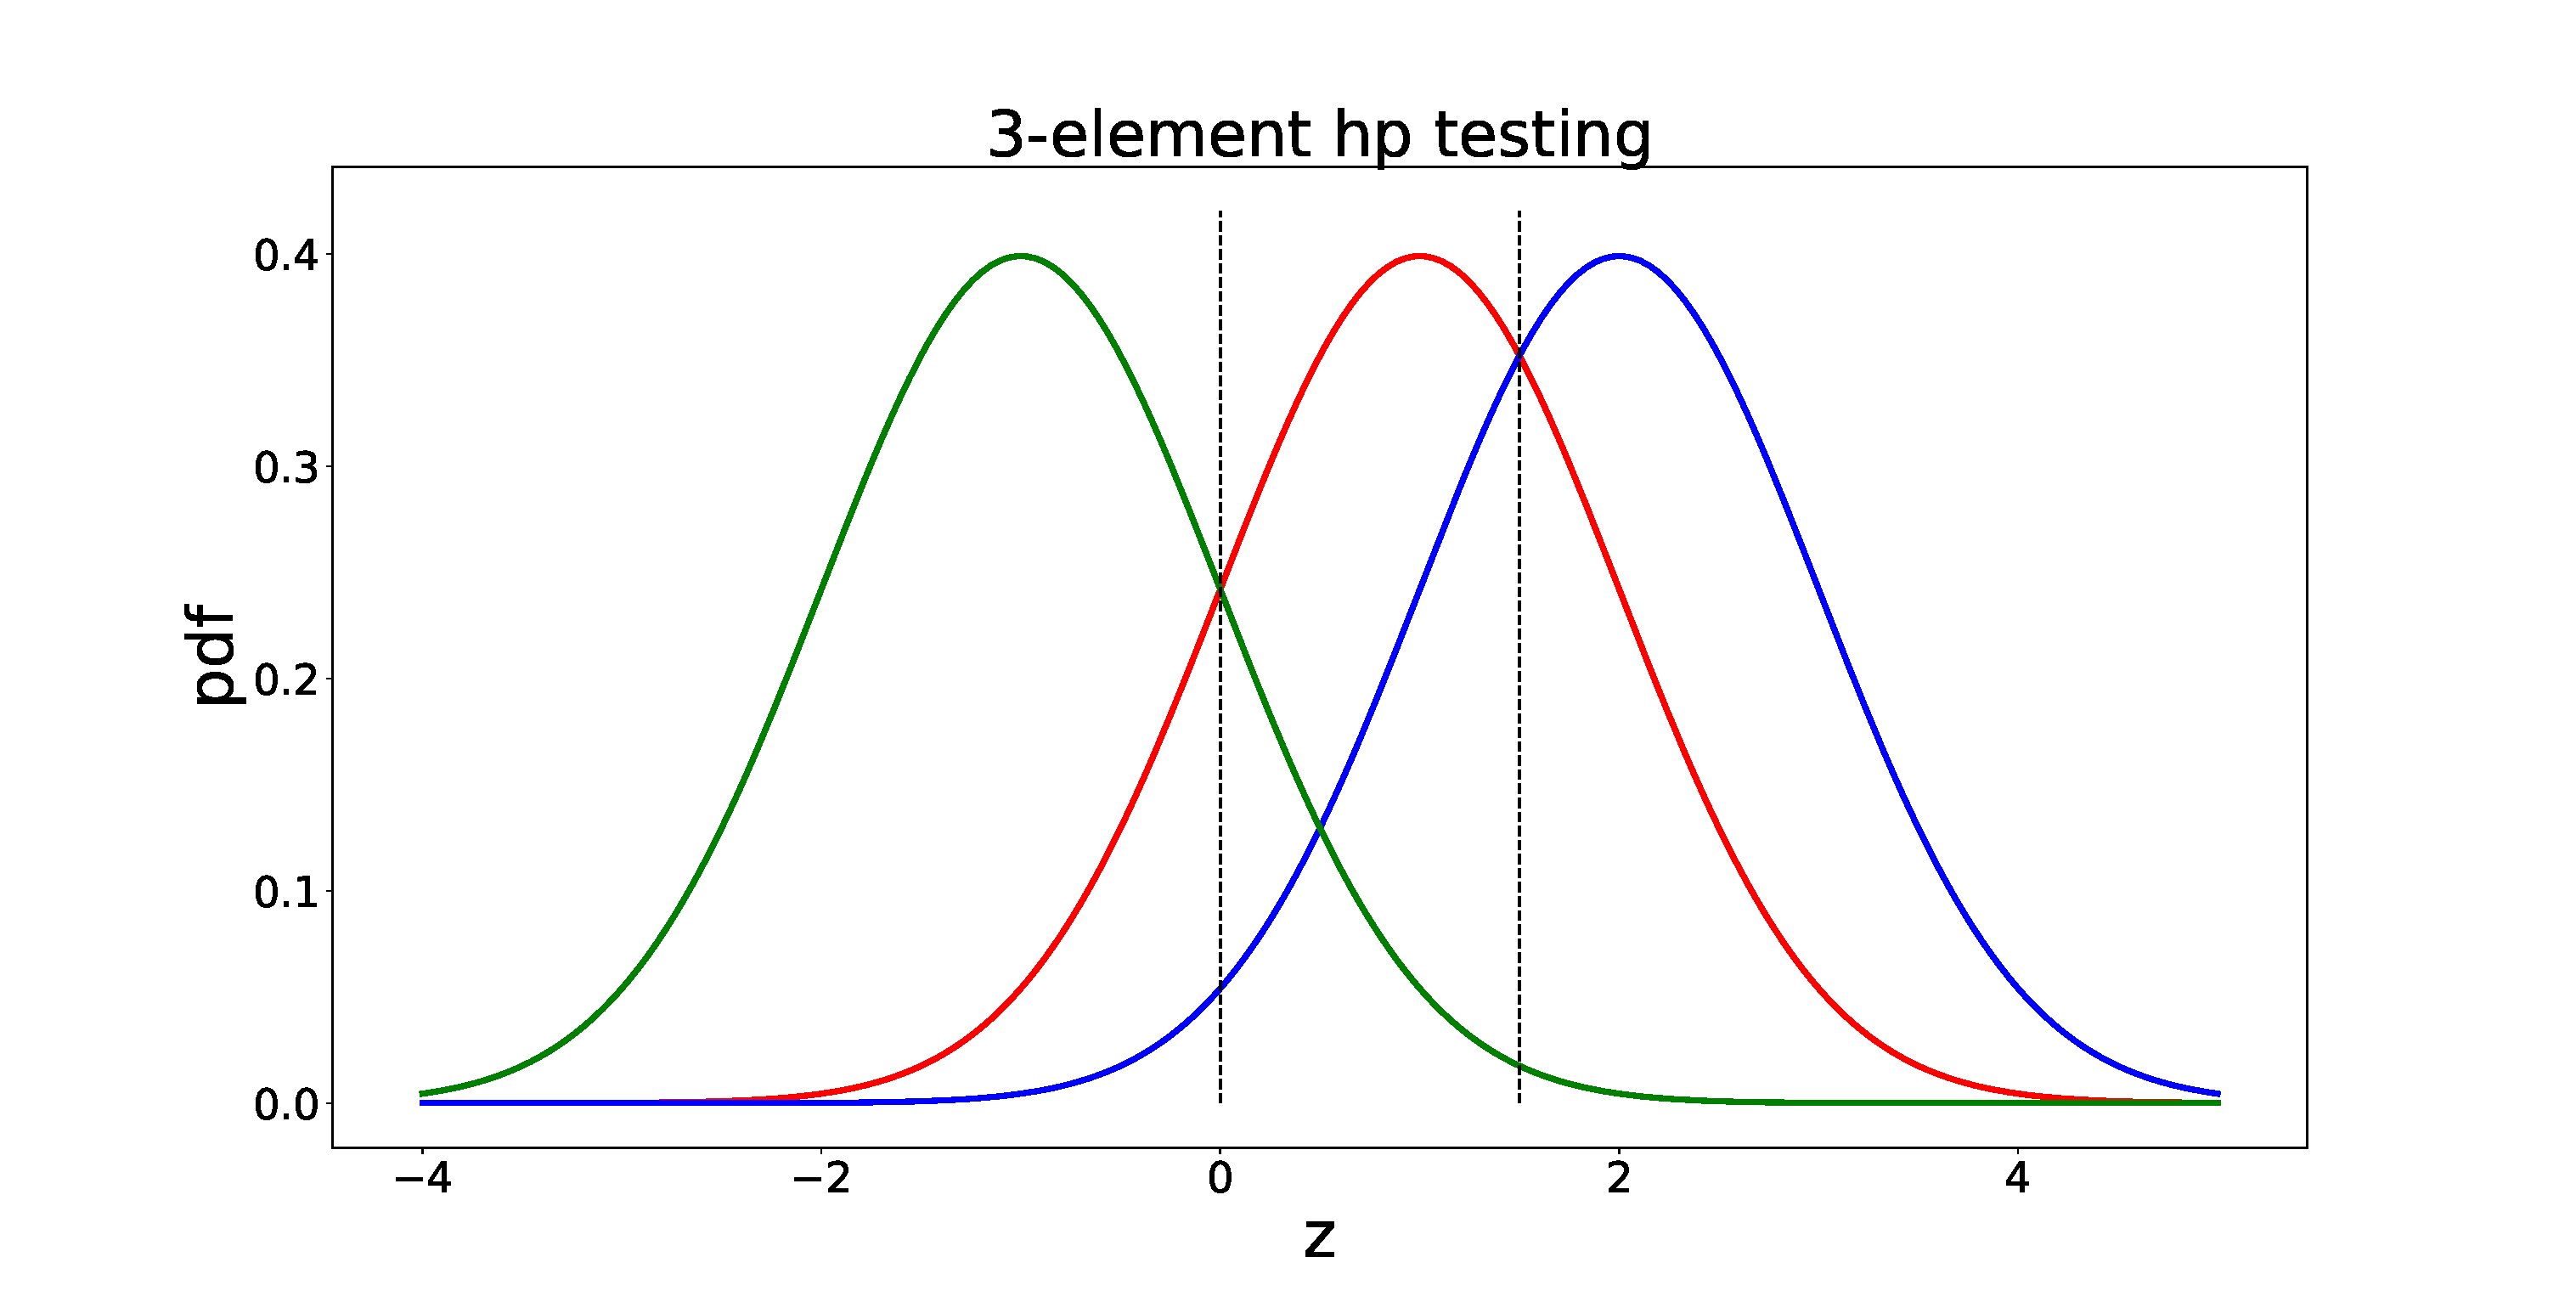
\includegraphics[width=0.8\textwidth]{3meta_hpt.eps}
\caption{三元假设问题}\label{fig:3meta_hpt}
\end{figure}

\item 复合假设检验:参量是随机变量

\begin{enumerate}[label=(\alph*)]
\item 若参量的概率分布已知,可将条件似然函数对参量的分布取平均,按简单假设检验求解。
比如假设
\begin{align*}
H_0 & :  s_0(t)=0 \\
H_1 & :  s_1(t)=A, \text{where}: A\sim N(0,\sigma_A^2)
\end{align*}
信道是高斯信道,观测$z(t)=s(t)+n(t)$, $n(t)\sim N(0,\sigma_N^2)$,且$A$与$n(t)$相互独立。
设只有1次观测, 
$z|H_0 \sim N(0,\sigma_N^2)$而
$$
p(z|H_1) = \int_{\mathbb{R}} p(z|H_1,A)p(A)dA=\frac{1}{\sqrt{2\pi (\sigma_N^2+\sigma_A^2)}} \exp(-\frac{z^2}{2(\sigma_N^2+\sigma_A^2)})
$$
$\Rightarrow z|H_1 \sim N(0,\sigma_N^2+\sigma_A^2)$
再通过似然比检验得到双边检验的形式:
$$
z^2 \mathop{\gtreqless}_{z\in \mathcal{Z}_0}^{z \in \mathcal{Z}_1} \frac{2\sigma_N^2(\sigma_A^2+\sigma_N^2)}{\sigma_A^2}\left[\ln \lambda_B + \frac{1}{2}\ln(1+\frac{\sigma_A^2}{\sigma_N^2})\right]
$$
\item 随机相位信号的检测
\begin{align*}
H_0 & :  z(t)=n(t),0\leq t\leq T,n(t)\text{是均值为0,谱密度为$\frac{N_0}{2}$的高斯白噪声} \\
H_1 & :  z(t)=\sqrt{\frac{2E_s}{T}}\sin(\omega_c t +\theta)+n(t), \text{where}: \\
& A\sim N(0,\sigma_A^2),\theta \text{是随机变量,$E_s$是该信号的能量}
\end{align*}
若$\theta$给定,假定$T$是$\frac{2\pi}{\omega_c}$的整数倍,可求出条件似然比为:
\begin{equation}
\lambda(z(t)|\theta) = \exp\left(\frac{2}{N_0}\sqrt{\frac{2E_s}{T}}(y_c \sin\theta + y_s \cos\theta)-\frac{E_s}{N_0}\right)
\end{equation}
其中:
\begin{align}
y_c & = \int_0^T z(t)\cos\omega_c t dt \\
y_s & = \int_0^T z(t)\sin\omega_c t dt \\
\end{align}
进一步假定随机相位$\theta$在$[0,2\pi]$区间上是均匀分布(最不利分布),则平均似然比为
\begin{align}
\lambda(z(t)) & = \E_{\theta}[\lambda(z(t)|\theta)] \\
               & = \exp(-\frac{E_s}{N_0})I_0(\frac{2}{N_0}\sqrt{\frac{2E_s}{T}}\sqrt{y_c^2+y_s^2}) \label{eq:ramdom_phase_LR}
\end{align}
其中
$$
I_0(x) = \frac{1}{2\pi}\int_0^{2\pi}\exp(x\cos\phi)d\phi
$$
称为零阶修正的Bessel 函数。
% from scipy.special import iv
% iv(0,x) is the function required
设 $ y = \sqrt{y_c^2 + y_s^2} $,由似然比判决规则可以得到
$$
y \mathop{\gtrless}_{H_0}^{H_1} y_T
$$

可以计算出$y$的概率密度函数为:
\begin{align}
p(y | H_1) & = \frac{y}{\sigma^2} \exp\left(-\frac{1}{2\sigma^2}\left[y^2+\frac{E_sT}{2}\right]\right)\cdot I_0\left(\frac{y}{\sigma^2}\sqrt{\frac{E_sT}{2}}\right) \\
p(y | H_0) & = \frac{y}{\sigma^2} \exp\left(-\frac{y^2}{2\sigma^2}\right)
\end{align}
其中$y>0,\sigma^2=\frac{N_0 T}{4}$,$y|H_0$服从Rayleigh 分布,是假设$H_1$下信号能量为0的特殊情况。

从而求出虚警概率$P_F$和检测概率$P_D$:
\begin{align}
P_F & = \int_{y_T}^{\infty} p(y|H_0)dy = \exp\left(-\frac{1}{2}\frac{y_T^2}{\sigma^2}\right) \\
P_D & = \int_{y_T}^{\infty} p(y|H_1)dy = Q\left(\frac{1}{\sigma}\sqrt{\frac{E_s T}{2}},\frac{y_T}{\sigma}\right)\label{eq:random_signal_PD}
\end{align}
其中
$$
Q(a,b) = \int_b^{\infty} u\exp\left(-\frac{u^2+a^2}{2}\right)I_0(au)du
$$
称为Marcum 函数。

采用 Neyman-Pearson 准则,由 $P_F =\alpha $ 得到$P_D=Q(\sqrt{\frac{2E_s}{N_0}},\sqrt{-2\ln \alpha})$。
信噪比$r=\frac{2E_s}{N_0}$,于是可作出接收机的ROC曲线以及当$\alpha$一定时检测概率与信噪比的关系曲线如图\ref{fig:ROC_random_phase_P_D_sim_SNR}所示。

\begin{figure}[!ht]
\centering
\begin{subfigure}{0.45\textwidth}
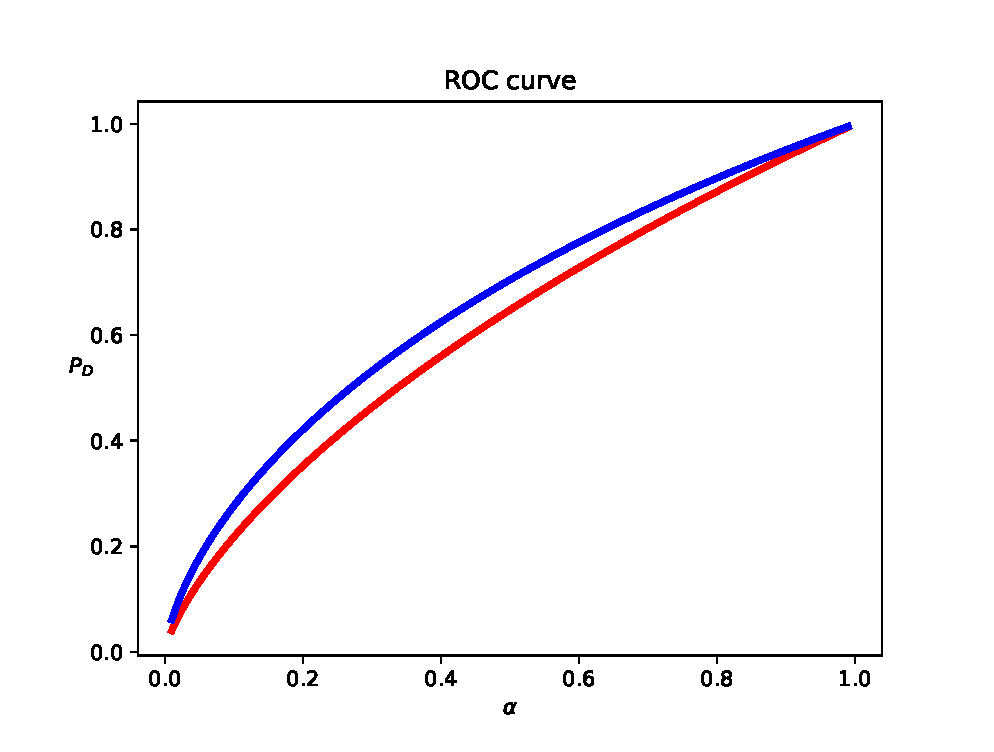
\includegraphics[width=\textwidth]{ROC_random_phase.eps}
\end{subfigure}~
\begin{subfigure}{0.45\textwidth}
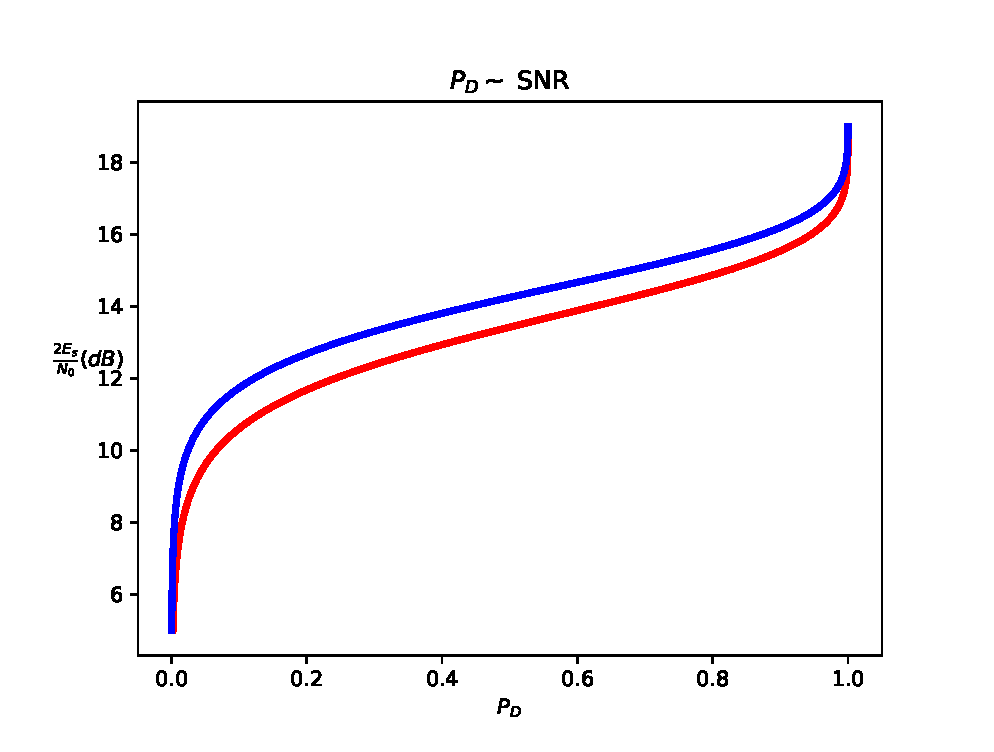
\includegraphics[width=\textwidth]{P_D_sim_SNR.eps}
\end{subfigure}
\caption{}\label{fig:ROC_random_phase_P_D_sim_SNR}
\end{figure}
% implementation scipy.stats.ncx2
% 1-ncx2.cdf(b^2,df=2,nc=a^2)
\item 随机幅度和相位信号的检测
\begin{align*}
H_0 & :  z(t)=n(t),0\leq t\leq T \\
H_1 & :  z(t)=A\sin(\omega_c t +\theta)+n(t), 0 \leq t \leq T
\end{align*}
$A$服从Rayleigh 分布:
$$
p(A)=\frac{A}{\sigma_A^2}\exp\left(-\frac{A^2}{2\sigma_A^2}\right),A \geq 0
$$
此时似然比为
$$
\lambda(z(t)) = \int_{0}^{\infty} \lambda(z(t) | A)p(A)dA
$$
其中$\lambda(z(t) |A)$可由 \eqref{eq:ramdom_phase_LR}得到为
$$
\lambda (z(t) | A) = \exp\left(-\frac{A^2 T}{2N_0}\right) \cdot I_0(\frac{2}{N_0}Ay)
$$
利用Marcum 函数的性质可得
$$
\lambda(z(t)) = \frac{N_0}{\sigma_A^2 T + N_0} \exp\left( \frac{2\sigma_A^2}{N_0(\sigma_A^2 T + N_0)}y^2 \right)
$$
再根据似然比检验的准则得到最佳接收机。

在随机相位、随机幅度的情况下,虚警概率$P_F$的计算与之前相同,而检测概率$P_D$则为\eqref{eq:random_signal_PD}对$p(A)$的平均(将$E_s=\frac{A^2 T}{2}$代入该式)。
可得:
\begin{equation}
P_D = \exp\left( -\frac{1}{2} \left(\frac{y_T}{2}\right)^2 \left(1+\frac{\bar{E}_s}{N_0}\right)^{-1}\right)
\end{equation}
其中$\bar{E}_s=\sigma_A^2 T$表示平均能量,$\bar{r}=\frac{\bar{E}_s}{N_0}$表示平均信噪比。
若令$P_F=\alpha$,则$P_D = \alpha^{1/(1+\bar{r})}$
\end{enumerate}
\item 色高斯信道

考虑一般的情形,噪声仍为高斯过程,但相关函数不再是$\delta{\tau}$而是一般的$R_n(t_1,t_2)$,可能是时变的。处理这一问题
可以用 Karhunen-Loeve 正交展开或者白化滤波器的方法。不同于白高斯信道中平均错误概率只与信号能量有关,在一般的色高斯信道中与信号波形有关。
\begin{enumerate}[label=(\alph*)]
\item 正交展开

把$z(t)$在基函数$\{g_k(t)\}$ 上展开:
\begin{equation}\label{eq:ztk}
z(t)= \sum_{k=1}^{\infty} z_k g_k(t), \text{where } z_k = \int_0^T z(t)g_k(t)dt
\end{equation}
展开的目的是希望选择基函数使得展开系数 $\{z_k\}$ 相互独立,因为$z_k$ 是高斯变量,所以只需使$\{z_k\}$ 互不相关即可,其协方差函数满足:
\begin{align}\notag
\Cov(z_k,z_l) & = \E\left[\int_0^T\int_0^T n(t_1)n(t_2)g_k(t_1)g_k(t_2)dt_1dt_2\right] \\
               & = \int_0^T\int_0^T R_n(t_1,t_2)g_k(t_1)g_k(t_2)dt_1dt_2
\end{align}
若
\begin{equation}
\int_0^T R_n(t_1,t_2)g_k(t_2)=\lambda_k g_k(t_1)
\end{equation}
且$\{g_k(t)\}$ 是归一化的正交函数集:
$$
\int_0^T g_k(t)g_l(t) = \delta_{kl}
$$
则 $\Cov(z_k,z_l)=\lambda_k \delta_{kl}$

似然比计算及判决规则:
我们以接收信号$K-L$展开式的前$N$个系数来建立“等效”的观测向量:$\bm{z}_N = (z_1,\dots,z_N)$。
似然比函数为
$$
\lambda(\bm{z}_N) = \frac{\prod_{k=1}^N \frac{1}{\sqrt{2\pi \lambda_k}} \exp\left(-\frac{(z_k-s_{1k})^2}{2\lambda_k}\right)}{\prod_{k=1}^N \frac{1}{\sqrt{2\pi \lambda_k}} \exp\left(-\frac{(z_k-s_{0k})^2}{2\lambda_k}\right)}
$$
其中 
\begin{equation}\label{eq:sik}
s_{ik}= \int_0^T s_i(t)g_k(t)dt,i=1,2
\end{equation}
是$z_k$的均值。
上式取对数并整理得:
$$
\ln \lambda(\bm{z}_N) = \sum_{k=1}^N \frac{1}{\lambda_k} z_k(s_{1k}-s_{0k}) - \frac{1}{2} \sum_{k=1}^{\infty} \frac{1}{\lambda_k} (s_{1k}^2 -s_{0k}^2)
$$
令 $N\to\infty$ 并将\eqref{eq:ztk}代入上式的第一项,\eqref{eq:sik}取一个代入上式第二项,得到:
\footnotesize
\begin{align*}
\ln \lambda(z(t)) & = \int_0^T z(t)\sum_{k=1}^{\infty} \frac{1}{\lambda_k} (s_{1k}-s_{0k})g_k(t)dt - \frac{1}{2}\left[\int_0^T s_1(t)\sum_{k=1}^{\infty} \frac{1}{\lambda_k} s_{1k}g_k(t)dt - \int_0^T s_1(t)\sum_{k=1}^{\infty} \frac{1}{\lambda_k} s_{0k}g_k(t)dt \right] \\
 & = \left[\int_0^T z(t) h_1(t)dt - \int_0^T z(t) h_0(t)dt\right] - \frac{1}{2}\left[\int_0^T s_1(t) h_1(t)dt - \int_0^T s_0(t) h_0(t)dt\right]
\end{align*}
\normalsize
其中 $h_i(t) = \sum_{k=1}^\infty \frac{1}{\lambda_k} s_{ik}g_k(t)$
易验证,$h_i(t)$ 是积分方程 $\int_0^T R_n(t,\tau)h_i(\tau)d\tau = s_i(t)$ 的解。
根据似然比检验准则有:
\small
\begin{equation}
\int_0^T z(t) h_1(t)dt - \int_0^T z(t) h_0(t)dt \mathop{\gtrless}_{H_0}^{H_1} v_T,\text{where } v_T=\ln \lambda_T + \frac{1}{2}\left[\int_0^T s_1(t) h_1(t)dt - \int_0^T s_0(t) h_0(t)dt\right]
\end{equation}
\normalsize
\item 白化滤波器

将接收信号$z(t)$通过一个滤波器$h_w(t,\tau)$,设输出信号为$z_w(t)$,则:
\begin{equation}
z_w(t) = \int_0^T h_w(t,\tau)z(\tau)d\tau | H_i = s_{wi}(t) + n_w(t)
\end{equation}
其中
\begin{align*}
s_{wi}(t) & = \int_0^T h_w(t,\tau)s_i(\tau)d\tau \\
n_w(t) & = \int_0^T h_w(t,\tau)n(\tau)d\tau
\end{align*}
若输出噪声$n_w(t)$是白噪声,则可以根据\eqref{eq:continuous_judge}的判决准则设计接收机。

假设$h_w(t,\tau)$可以展开为:
$$
h_w(t,\tau) = \sum_{k=1}^{\infty} h_k g_k(t) g_k(\tau)
$$
于是可得:
\begin{align*}
R_{n_w}(t,\tau) & = \E[n_w(t)n_w(\tau)]\\
                & = \E\left[\int_0^T\int_0^T h_w(t,s)h_w(\tau,u)n(s)n(u)dsdu\right]\\
                & = \int_0^T\int_0^T h_w(t,s)h_w(\tau,u)R_n(s,u)dsdu \\
                & = \int_0^T\int_0^T \left[\sum_{k=1}^{\infty} h_k g_k(t) g_k(s)\right]\left[\sum_{l=1}^{\infty} h_l g_l(\tau) g_l(u)\right]R_n(s,u)dsdu \\
                & = \sum_{k=1}^{\infty}\sum_{l=1}^{\infty}\int_0^T  h_k g_k(t) g_k(s) h_l g_l(\tau) \lambda_l g_l(s)ds \\
                & = \sum_{k=1}^{\infty}\sum_{l=1}^{\infty} h_k g_k(t)  h_l g_l(\tau) \lambda_l\delta_lk \\
                & = \sum_{k=1}^{\infty} \lambda_kh^2_k g_k(t)g_k(\tau)  \\
\end{align*}
另一方面
$$
\delta(t-\tau) = \sum_{k=1}^{\infty} g_k(t)g_k(\tau)
$$
比较系数得:
\begin{equation}
h_k = \frac{1}{\sqrt{\lambda_k}} \Rightarrow h_w(t,\tau) = \sum_{k=1}^{\infty} \frac{1}{\sqrt{\lambda_k}} g_k(t)g_k(\tau)
\end{equation}
\end{enumerate}
\item 练习题
\begin{enumerate}[label=(\arabic*)]
\item 试推导如下情况的似然比。
\begin{align*}
H_0 & :  z\sim N(m_0,\sigma_0^2) \\
H_1 & :  z\sim N(m_1,\sigma_1^2)
\end{align*}
并求判决域和错误概率。
\begin{proof}[解]
\begin{align}
\lambda(z) = & \frac{p(z|H_1)}{p(z|H_0)} \\
            = & \frac{\sigma_0}{\sigma_1}\exp(-\frac{(z-m_1)^2}{2\sigma_1^2}+\frac{(z-m_0)^2}{2\sigma_0^2})\label{eq:Gaussian_likelyhood_ratio}
\end{align}
\begin{align*}
\mathcal{Z}_0 = & \{z|\lambda(z) < \lambda_B\} \\
= & \{z| (\sigma_1^2-\sigma_0^2)z^2-2(m_0\sigma_1^2-m_1\sigma_0^2 +m_0^2 \sigma_1^2-m_1^2\sigma_0^2<2\sigma_0^2\sigma_1^2(\ln \lambda_B - \ln {\sigma_0 \over \sigma_1})) \}\\
\mathcal{Z}_1 = & \{z|\lambda(z) > \lambda_B\}
\end{align*}
\begin{align*}
P_F = P(D_1,H_0) = & \int_{z\in \mathcal{Z}_1} p(z|H_0)dz \\
P_M = P(D_0,H_1) = & \int_{z\in \mathcal{Z}_0} p(z|H_1)dz 
\end{align*}
Discuss $\sigma_1 \gtreqless \sigma_0,m_1\gtreqless m_0$.
\end{proof}
\item 考虑一二元对称信道,$\epsilon$是交叉概率(假定$\epsilon< \frac{1}{2}$),即信道输入为0(或1)时,输出为$b$(或$a$)的概率。若先验概率相等,试导出保证
平均错误概率最小的判决准则,并求最小平均错误概率。
\begin{proof}[解]
考虑一次观测$z$,
\begin{align*}
H_0 & :  \theta = 0 \\
H_1 & :  \theta = 1
\end{align*}
条件概率$z|\theta$已知:$p_{z|\theta=0}(a)=1-\epsilon,p_{z|\theta=0}(b)=\epsilon,p_{z|\theta=1}(a)=\epsilon,p_{z|\theta=1}(b)=1-\epsilon$
由似然比检验,$\lambda(z)=\frac{p(z|H_1)}{p(z|H_0)}\Rightarrow \lambda(a)=\frac{\epsilon}{1-\epsilon}<1,\lambda(b)=\frac{\epsilon}{1-\epsilon}>1$
因为先验概率相等,所以$\lambda_B=1$,因此判决准则为$z=b \Rightarrow \theta=1; z=a\Rightarrow \theta=0$。
平均错误概率为
\begin{align*}
P_{\theta,z}(0,b)+P_{\theta,z}(1,a)= & P_{\theta}(0) P_{z|\theta=0}(b) + P_{\theta}(1) P_{z|\theta=1}(a) \\
                                 = & \epsilon 
\end{align*}
或比较四类判决的错误概率,分别为$\epsilon,{1\over 2},{1\over 2},1-\epsilon$。
\end{proof}
\item 请使用最小错误概率准则,设计一个在如下两种假设间作出选择的接收机(假定两种假设的先验概率相等):
\begin{align*}
H_0 & :  z(t) = s_0(t) + n(t) \\
H_1 & :  z(t) = s_1(t) + n(t)
\end{align*}
其中:信号$s_1(t)$ 和 $s_0(t)$如图\ref{fig:13}所示:噪声$n(t)$ 是高斯型随机变量,均值为零,谱密度为$\frac{N_0}{2}$。并画出平均错误概率与$\frac{2E}{N_0}$的函数关系($E$为信号的平均能量)。
\begin{figure}[!ht]
\centering
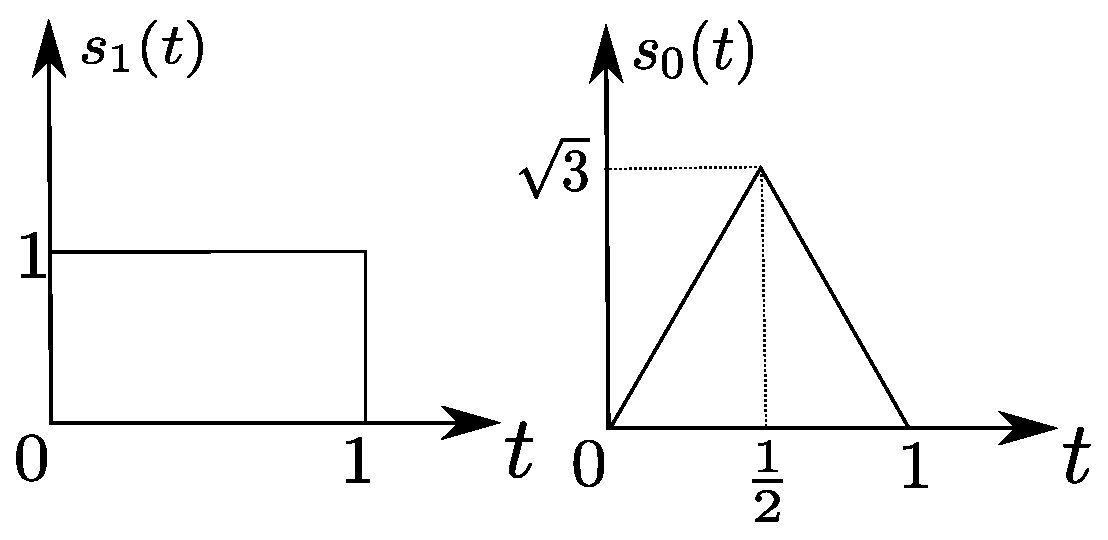
\includegraphics[width=0.7\textwidth]{practice_13.eps}
\caption{信号$s_1(t)$ 和 $s_0(t)$}\label{fig:13}
\end{figure}
\begin{proof}[解]
首先计算信号的能量 $E_1=1,E_2=1,\mathscr{L}_T=1\Rightarrow v_T=0$,根据\eqref{eq:continuous_judge}式可得到最小错误概率的判决准则。
$s_1(t)$和$s_2(t)$的互相关系数$\rho=\frac{\sqrt{3}}{2}$。
由\eqref{eq:continuous_eq_prob}式可得到平均错误概率为
$$
\bar{R}=\frac{1}{2}(P_F+P_M)=\Phi\left(-\sqrt{\frac{2E}{N_0}\left(\frac{1}{2}-\frac{\sqrt{3}}{4}\right)}\right)
$$
平均错误概率与$\frac{2E}{N_0}$的函数关系如图\ref{fig:average_error_with_SNR}所示

\begin{figure}[!ht]
\centering
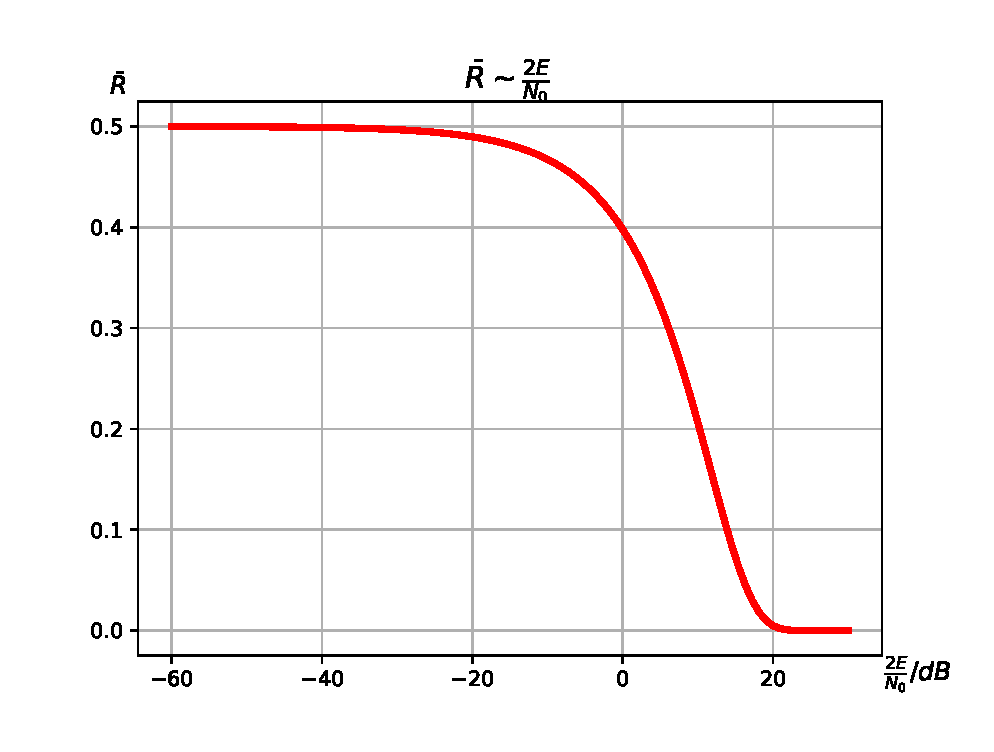
\includegraphics[width=0.7\textwidth]{average_error_with_SNR.eps}
\caption{}\label{fig:average_error_with_SNR}
\end{figure}
%frame on, use dB unit
\end{proof}
\item 已知$K$个独立的观测值

$\begin{cases}
H_1 : & z_k = n_k \\
H_0 : & z_k = 1 + n_k
\end{cases}$
其中:$n_k$是均值为零、方差为2的高斯随机变量,$k=1,2,\dots,K$。
\begin{enumerate}[label=(\alph*)]
\item 设计似然比检验,并求$P_F$和$P_M$。
\item 画出$K=1$时的接收机工作特性。
\item 假定$c_{00}=c_{11}=0,c_{01}=2,c_{10}=1,P(H_0)=0.7$,试求最小$N$值,使得$K=N$时的风险不大于$K=1$时风险的$\frac{1}{2}$。
\end{enumerate}
\begin{proof}[解]
\begin{enumerate}[label=(\alph*)]
\item 设$\bm{z}=[z_1,\dots,z_K],\lambda(\bm{z})=\frac{p(\bm{z}|H_1)}{p(\bm{z}|H_0)}$
$$
\lambda(\bm{z})\mathop{\gtreqless}_{H_0}^{H_1} \lambda_B \Rightarrow z \mathop{\gtreqless}_{H_1}^{H_0} \frac{1}{2}-\frac{2}{K}\ln \lambda_B
$$
其中$z=\frac{1}{K}\sum_{i=1}^K z_i,z|H_0 \sim N(1,\frac{2}{K}),z|H_1 \sim N(0,\frac{2}{K})$
\begin{align*}
P_F = & \int_{-\infty}^{\frac{1}{2}-\frac{2}{K}\ln \lambda_B} p(z|H_0)dz \\
    = & \Phi\left(-\sqrt{2K}(\frac{1}{4}+\frac{\ln \lambda_B}{K})\right) \\
P_M = & \Phi\left(-\sqrt{2K}(\frac{1}{4}-\frac{\ln \lambda_B}{K})\right)
\end{align*}
\item 当$K=1$时,以$\lambda_B$作为曲线参数,作出$(P_F,P_D)$的曲线如图\ref{fig:ROC_curve} 所示。

\begin{figure}[!ht]
\centering
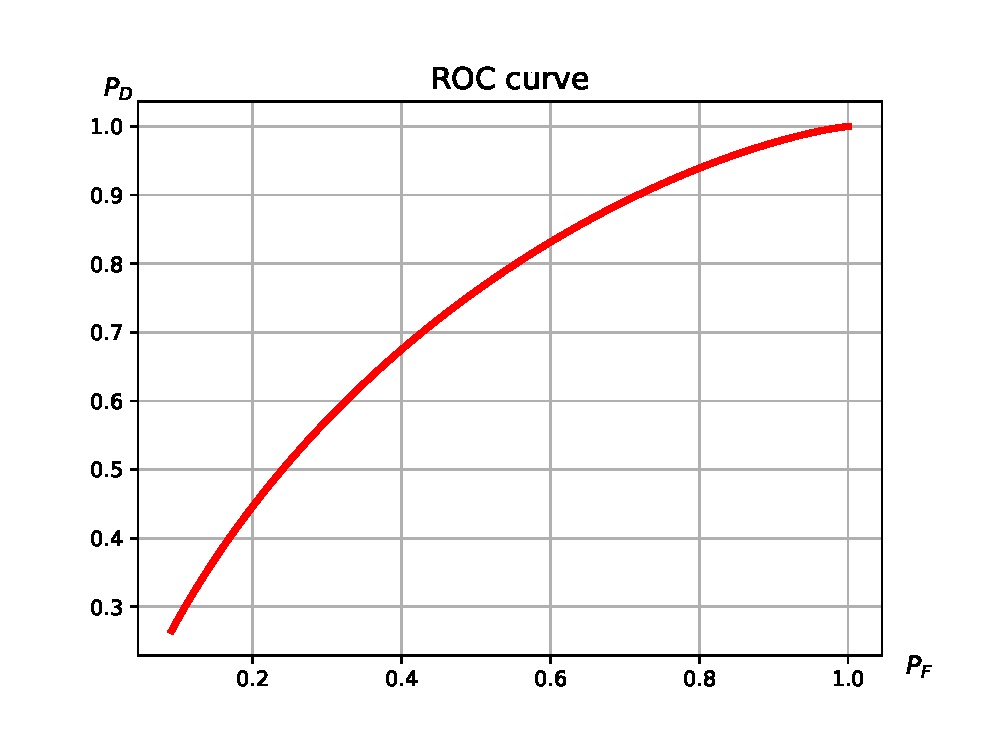
\includegraphics[width=0.7\textwidth]{ROC_curve.eps}
\caption{}\label{fig:ROC_curve}
\end{figure}

\item 
\begin{align*}
\bar{R} = & C_{01} P(D_0,H_1) + C_{10} P(D_1,H_0) \\
         = & 2 P(H_1) P(D_0 | H_1) + P(H_0) P(D_1 | H_0) \\
         = & 0.6 P_M + 0.7 P_F
\end{align*}
另一方面,
$$
\lambda_B = \frac{P(H_0)(C_{10}-C_{00})}{P(H_1)(C_{01}-C_{11})} = \frac{7}{6}
$$
根据(a)
$\bar{R}(K=1)=0.47,\bar{R}(K=6)=0.25,\bar{R}(K=7)=0.23 < \frac{1}{2}\bar{R}(K=1) \Rightarrow N=7$
\end{enumerate}
\end{proof}
\item 对于二元通信系统,其假设为:

$
\begin{cases}
H_1 : & z(t) = A\cos\omega_1 t + B \cos(\omega_2 t +\phi) + n(t)\\
H_0 : & z(t) = B\cos(\omega_2 t + \phi) + n(t)
\end{cases}
$其中:$\begin{array}{c}
0\leq t \leq T \\
A,B,\omega_1,\omega_2,\phi \textrm{ are known constant}
\end{array}$

假定: $\int_0^T \cos\omega_1 t \cos\omega_2 t dt = \int_0^T \cos\omega_1 t \sin\omega_2 t dt = 0, n(t)$ 是谱密度为$\frac{N_0}{2}$的高斯白噪声。试画出
其最佳接收机模型,并分析其误码率是否和$A\cos\omega_1 t $及$B\cos(\omega_2 t + \phi)$有关。计算误码率以证明你的分析结论。
\begin{proof}[解]
假定等先验概率,由\eqref{eq:continuous_eq_prob}得 
$$
P_e = \Phi(-\sqrt{\frac{E(1-\rho)}{N_0}})
$$
而
\begin{align*}
E(1-\rho) = & \frac{1}{2} \int_0^T (s_1(t)-s_0(t))^2 dt \\
          = &  \frac{1}{2} \int_0^T (A\cos\omega_1 t)^2 dt 
\end{align*}
因此误码率与$A\cos\omega_1 t$有关而和$B\cos(\omega_2 t + \phi)$无关。
\end{proof}
\end{enumerate}
\end{enumerate}

\end{document}



